\documentclass{article}
\usepackage[backend=biber]{biblatex}
\usepackage{graphicx}
\usepackage[colorlinks=true]{hyperref}
\usepackage{booktabs}
\usepackage{siunitx}
\usepackage[]{amsmath}
\usepackage{gensymb}
\usepackage{mathtools}
\usepackage{fancyref}
\addbibresource{/home/giorgio/Bibliography/bibliography.bib}
\hypersetup{
    colorlinks=true,
    linkcolor=blue,
    filecolor=magenta,  
    citecolor=blue,    
    urlcolor=cyan,
    pdftitle={Turbina ad alta temperatura},
    bookmarks=true,
}

\author{Giorgio De Trane, \\Anthony Steven Luna Gonzales, \\Giulia Barbero, \\Roberto Giusto}
\title{\textbf{Turbina ad alta temperatura}}

\begin{document}
    \setlength{\parindent}{0pt}
    \maketitle
    \begin{center}
        
\includegraphics[width=0.8\textwidth]{Sources/polito_logo.png}\linebreak\newline
       \textbf{\textit{Materiali per applicazioni aerospaziali}}\linebreak\newline
        \textit{Gruppo di lavoro n. 10B}\linebreak\newline
        \textit{Anno accademico 2020/2021}
    \end{center}

    \newpage
    \tableofcontents
    \newpage
    \section{Introduzione\label{Intro}}
    I turbomotori assiali aeronautici possono essere suddivisi, generalmente, in tre macrosezioni
    fondamentali: compressore, camera di combustione e turbina.\\

    \begin{figure}[h!]
        \centering
        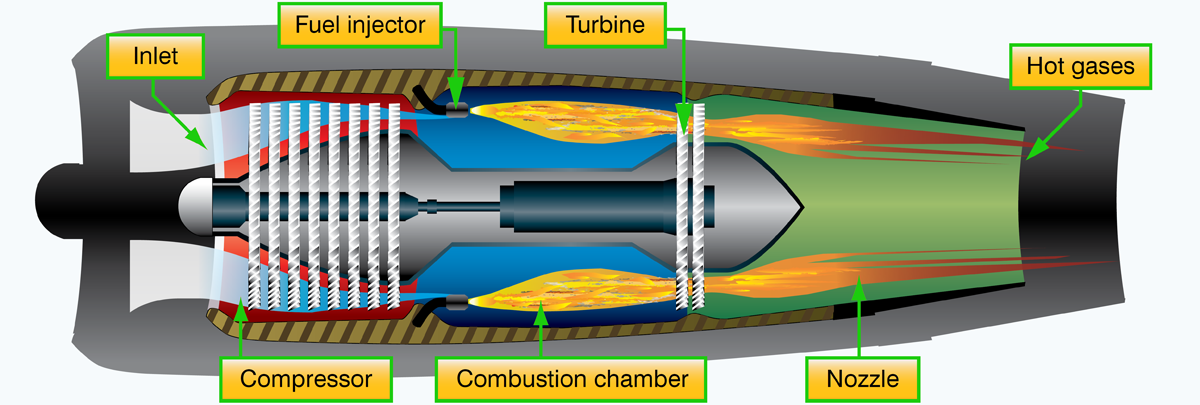
\includegraphics[width=0.8\textwidth]{Sources/turbojet.png}\\
    \caption{Schema generale di un motore turbojet \autocite*{turbojet}} 
    \end{figure}

    Un \textit{inlet} favorisce l'afflusso di aria esterna al \textit{compressore}, il quale
    la comprime in un volume nettamente inferiore, attraverso vari stadi alternati di pale rotoriche-statoriche.\\
    L'aria fortemente compressa viene poi miscelata con il carburante iniettato in \textit{camera di combustione},
    in una determinata proporzione (dipendente da vari fattori): la miscela viene quindi combusta, seguendo le trasformazioni di
    un preciso ciclo termodinamico (ogni motore ha la sua implementazione, ma i principi fondamentali sono gli stessi), causando un repentino
    aumento di pressione e temperatura.\\
    Successivamente, i gas combusti vengono espansi rapidamente dalla \textit{turbina} (la quale, inoltre, mette in rotazione l'albero di trasmissione), attraverso, in questo caso,
    vari stadi alternati di pale statoriche-rotoriche.\\
    Infine, i gas espansi vengono espulsi e accelerati attraverso un \textit{ugello}.\\
    Tutto il processo fornisce una spinta, secondo il principio di azione-reazione \autocite*{Aircr_engine_design}.\\ \\
    Le temperature e le sollecitazioni raggiunte dalle palette di turbina sono tipicamente in range estremi (in particolare per gli stadi ad alta pressione),
    al punto che la scelta dei materiali é sostanzialmente diversa da quella del compressore.\\
    In un moderno jet engine, si possono raggiungere temperature massime che eccedono i 1500 °C \autocite*{SciencePubGroup}, 
    senza contare le sollecitazioni meccaniche a cui sono sottoposte le pale HP, a causa di pressioni elevatissime,
    forze centrifughe per velocitá di migliaia di RPM e intense vibrazioni, nonché problemi di corrosione
    e reazioni chimiche indesiderate, favorite oltretutto dall'alta temperatura.\\

    \begin{figure}[h!]
        \centering
        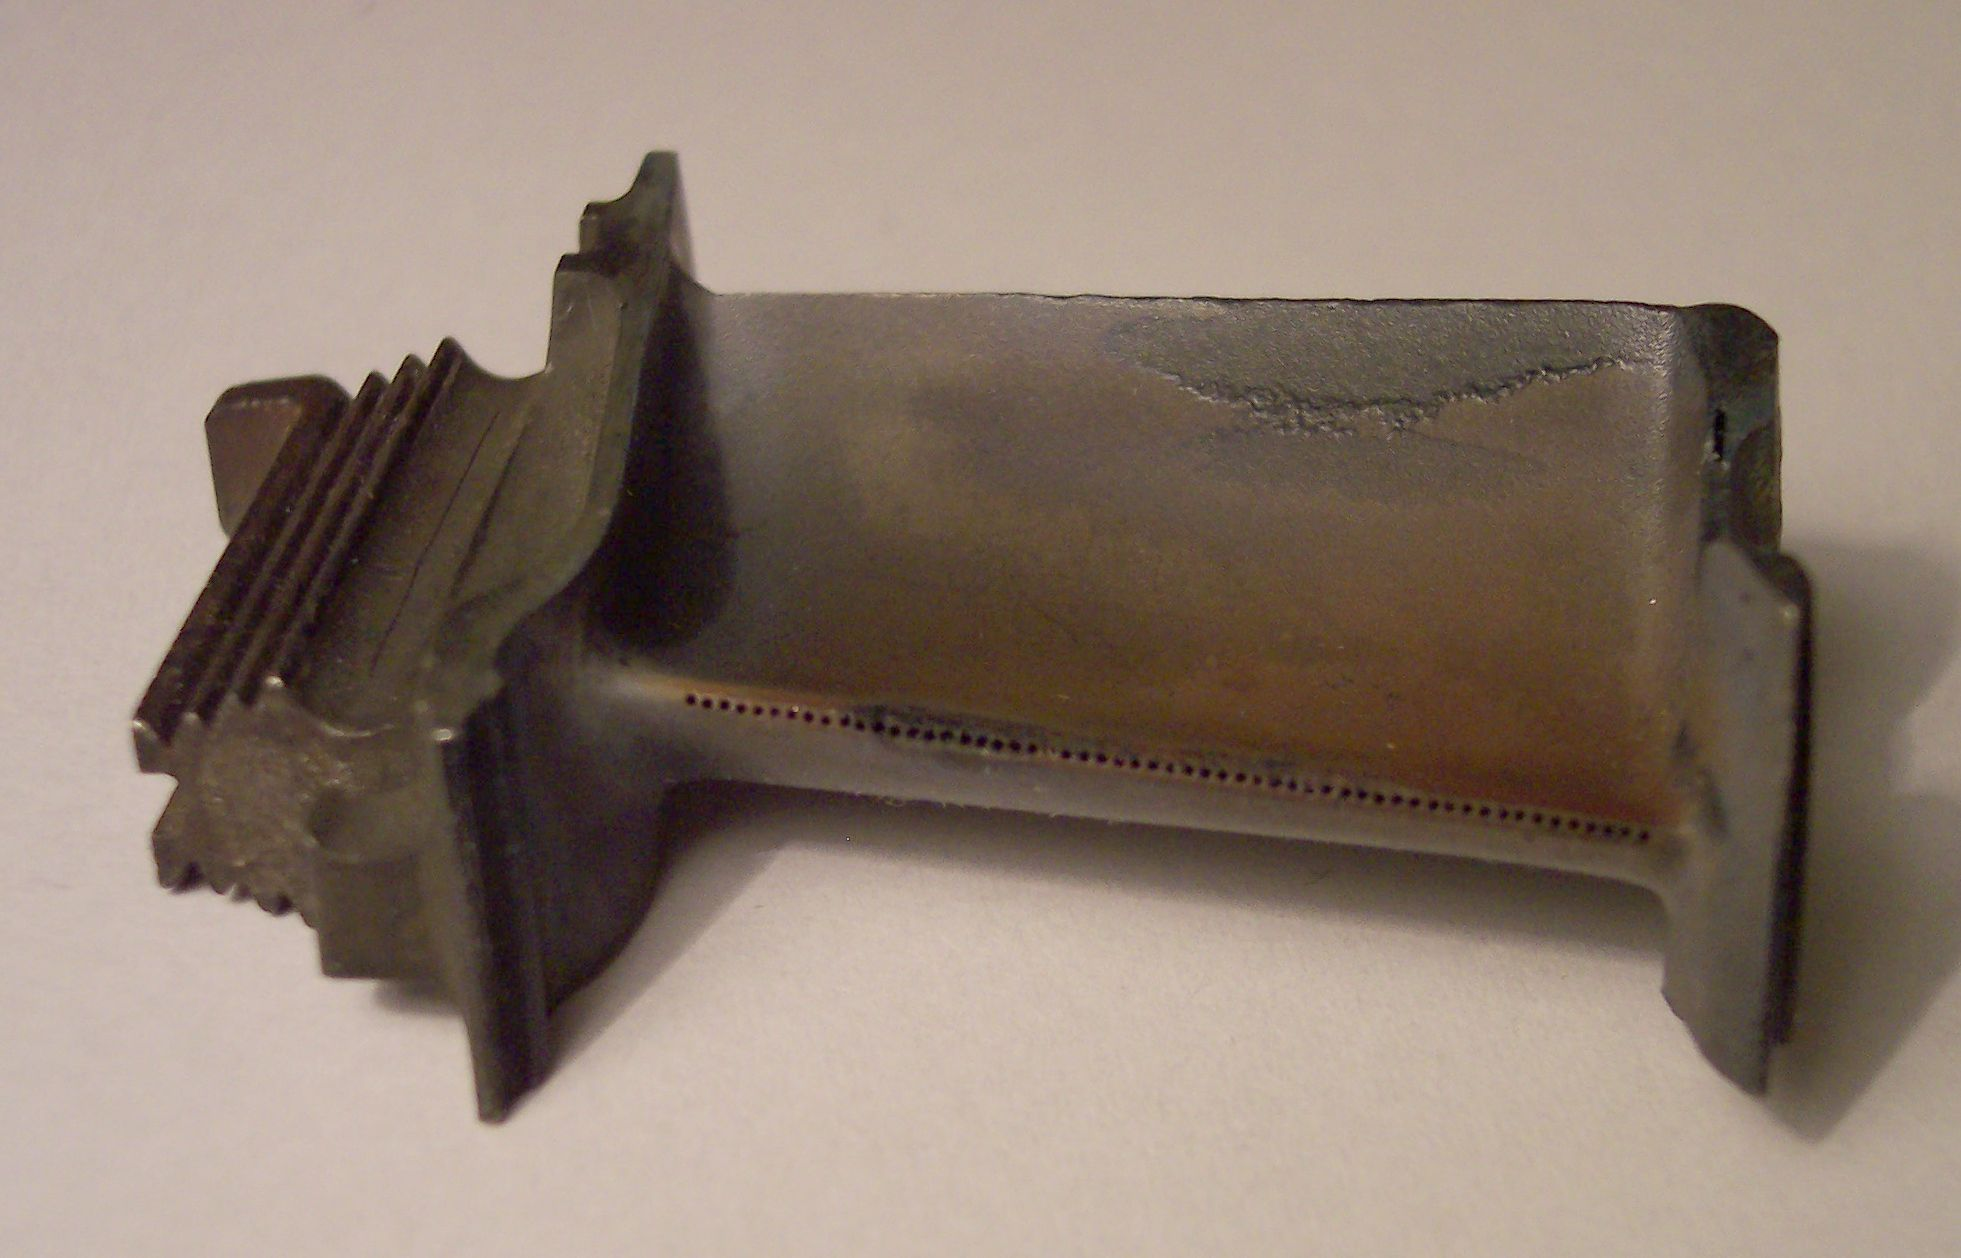
\includegraphics[width=\textwidth]{Sources/Turbinenschaufel_RB199.jpg}
        \caption{Effetti dell'ambiente operativo estremo su una paletta di turbina \autocite*{turbine_blade}}
        \phantomsection \label{fig:paletta_logorata}
    \end{figure}

    É necessario, dunque, scegliere un materiale (o una combinazione di piú materiali)
    in grado di sopportare, per il tempo di operativitá del componente, l'effetto
    simultaneo dell'elevatissima temperatura, dell'aggressivitá chimica e delle sollecitazioni meccaniche istantanee e cicliche,
    tenendo in considerazione, eventualmente, la possibilitá di un raffreddamento attivo.\\

    \clearpage




    \section{Superleghe nei motori aeronautici\label{superleghe_mot_aer}}
  
    L'evoluzione esponenziale del settore aerospaziale e di tutte le discipline satelliti, 
    nel corso degli ultimi decenni, vede sicuramente la scienza dei materiali 
    tra i suoi driving factors.

    Tra le infinite innovazioni, un ruolo essenziale é sicuramente giocato dalle \textit{superleghe}.

    Tali leghe metalliche sono cosí definite poiché possono tipicamente raggiungere
    una temperatura di esercizio pari a circa il 70-80 \% della propria temperatura di 
    fusione, anche per periodi piuttosto prolungati, pur mantenendo eccezionali
    proprietá meccaniche.
    \\ 

    In commercio sono disponibili una moltitudine di superleghe, tra cui quelle basate 
    sul Nickel, sul Titanio, sul Cobalto e molte altre.
    Viste le elevatissime temperature di esercizio delle palette di turbina HP, le
    uniche superleghe, con cui al momento sono prodotte, sono proprio quelle a base di Nickel. 
    
    \begin{figure}[h!]
        \centering
        \phantomsection \label{turbofan_drawing}
        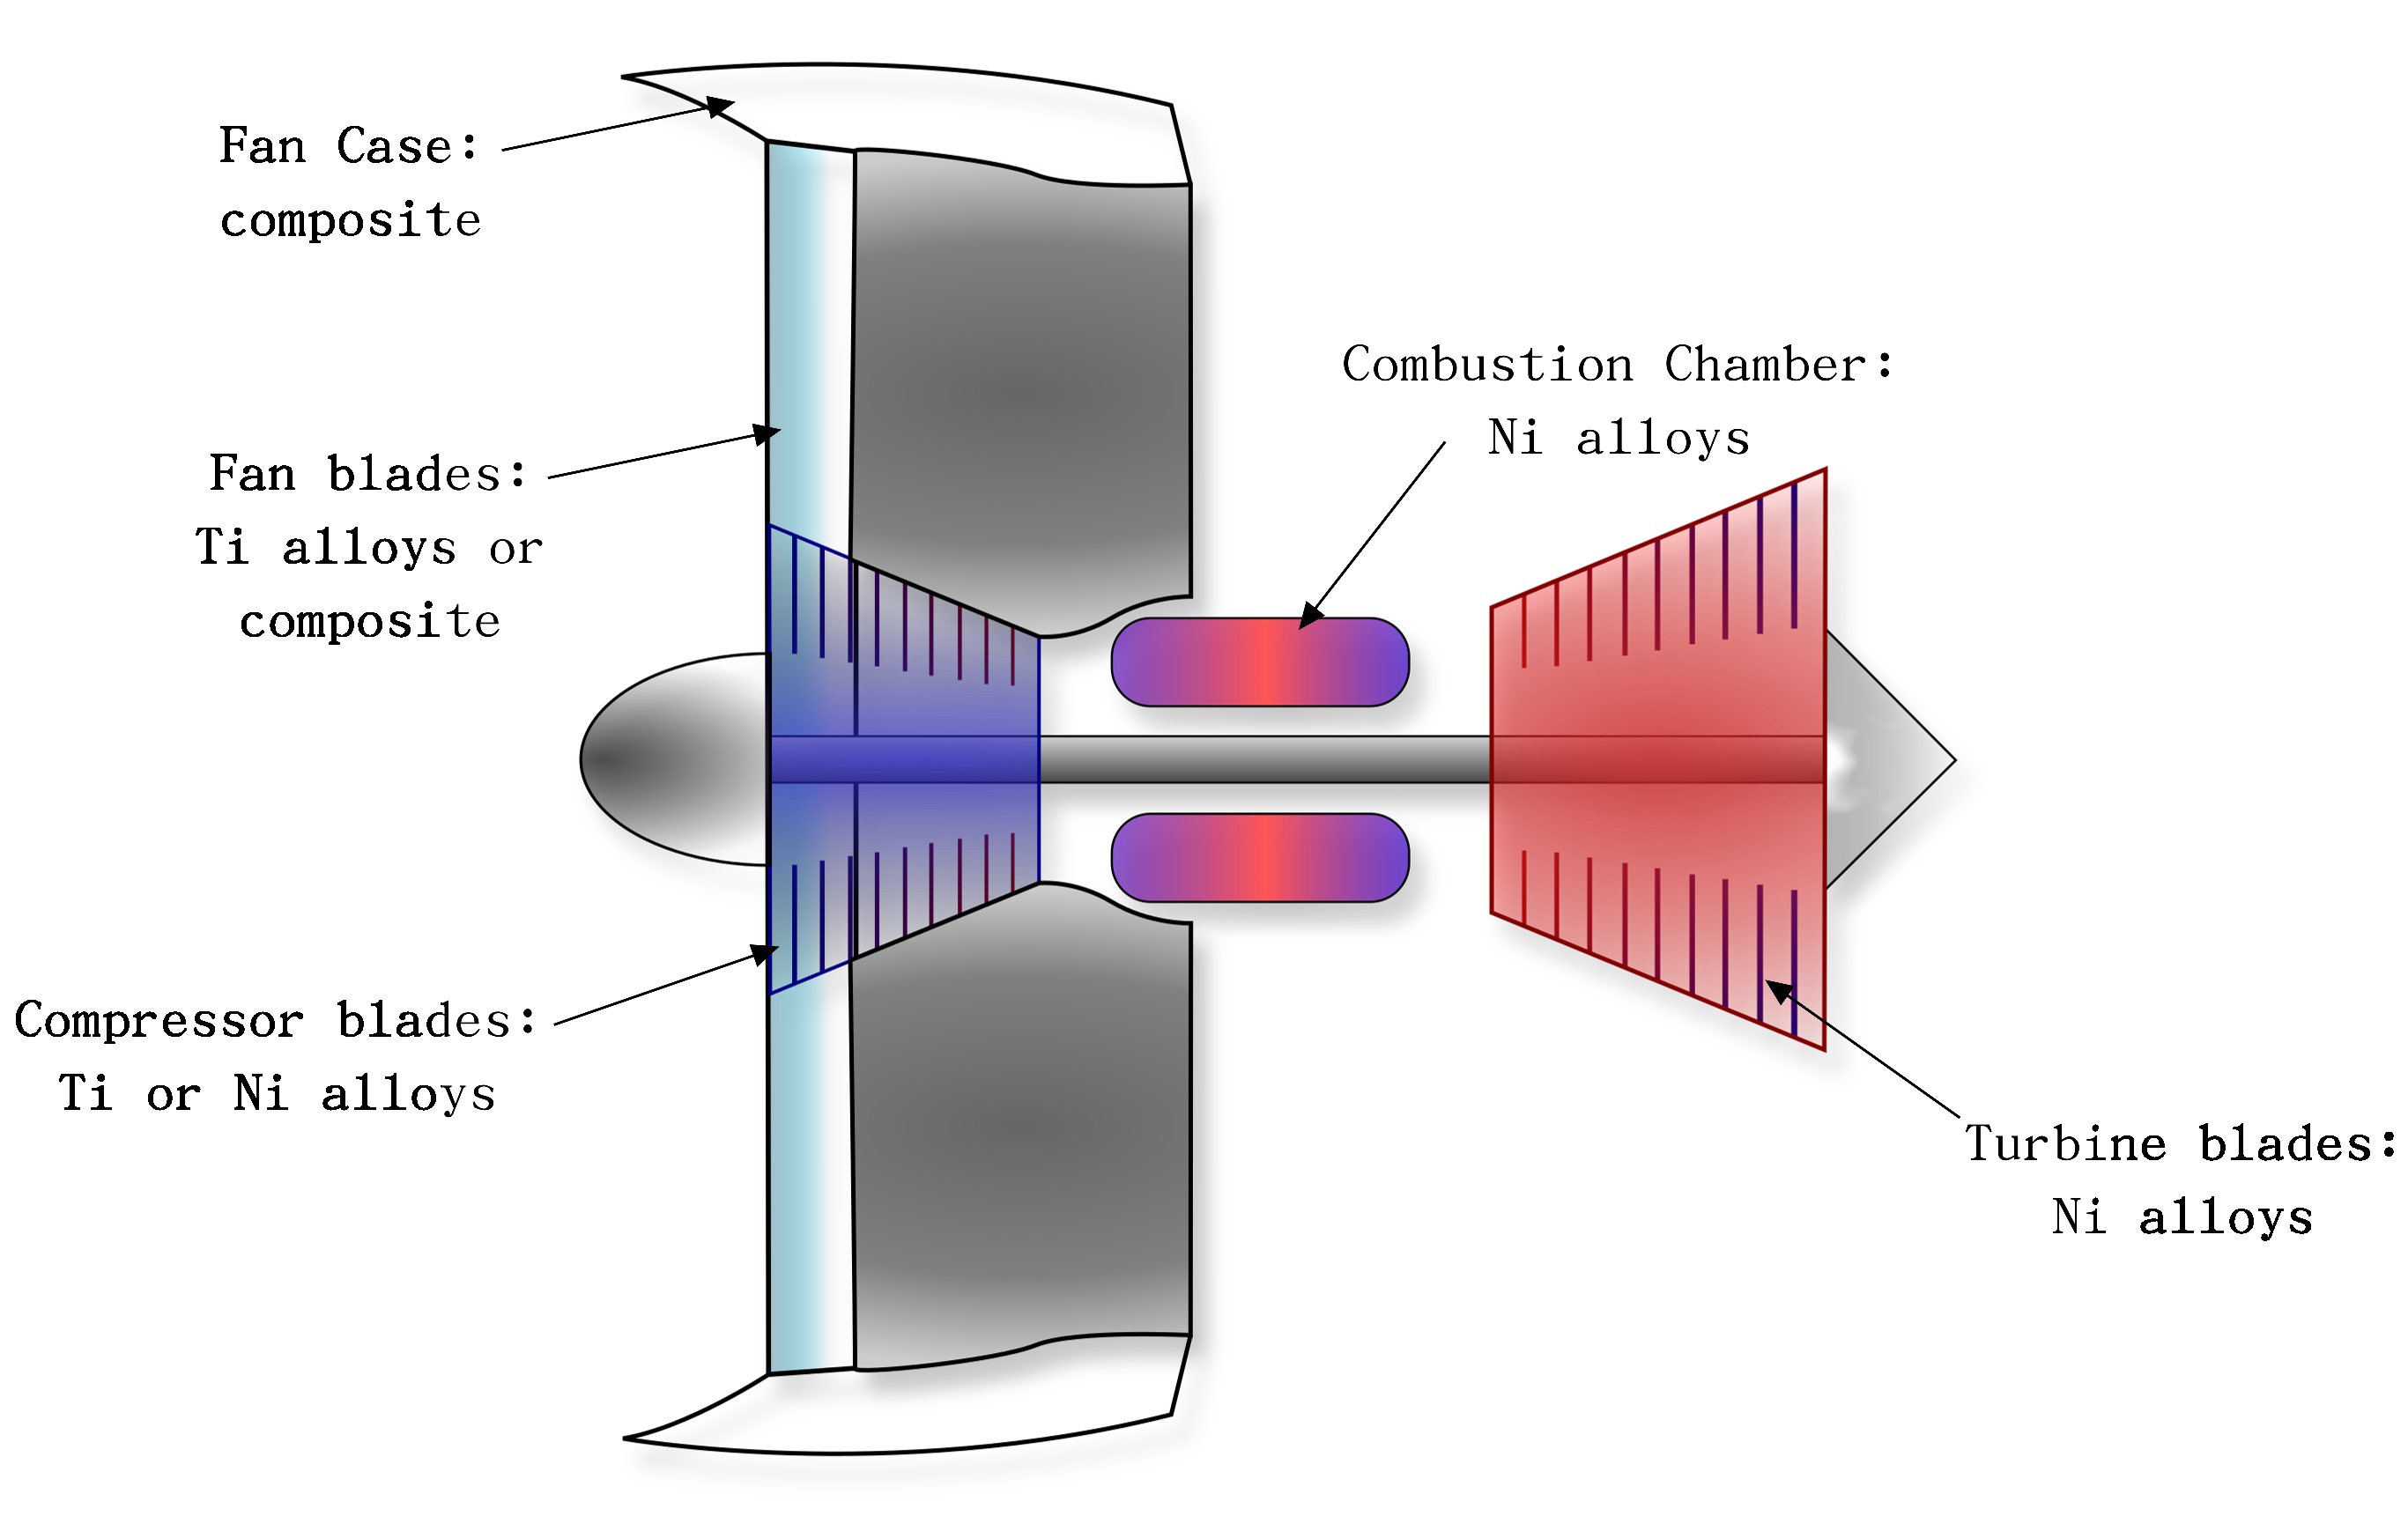
\includegraphics[width=0.95 \textwidth]{Sources/engine_drawing.eps}
        \caption{Materiali tipici in un motore turbofan \autocite{Inkscape}}
    \end{figure}

    Queste superleghe hanno portato innumerevoli benefici nell'efficienza operativa
    complessiva dei moderni velivoli.

    Ad esempio, all'aumentare del gradiente termico operativo, aumenta il rendimento del motore, 
    con un impatto positivo sull'efficienza e sui costi complessivi.

    Inoltre, l'elevata resistenza agli sforzi ciclici, a cui le palette sono 
    continuamente sottoposte, consente una riduzione e semplificazione delle invasive operazioni
    di manutenzione a terra, diminuendo quindi l'introduzione di errori umani e, allo stesso
    tempo, garantendo al velivolo un maggior numero di missioni durante la propria vita operativa.






    \clearpage

        \subsection{Composizione delle superleghe di Nickel\label{Nickel_composizione}}

        Una peculiaritá delle superleghe di Nickel é l'elevata presenza di elementi alliganti, fino 
        al 40-60\%, in una matrice di Nickel \autocite{Mouritz}. \\ 

        Sono tipicamente inseriti Cromo (10-20\%),
        Cobalto (5-15\%), Alluminio e Titanio (8\%, complessivamente), oltre
        a piccole quantitá di elementi
        come Molibdeno, Tungsteno e Carbonio. \\ \\ 

      
        \begin{table}[h!]
            \centering
            \resizebox{\textwidth}{!}{%
            \begin{tabular}{@{}cl@{}}
            \toprule
            \multicolumn{1}{l}{\textbf{Elemento}} & \textbf{Funzione}                                               \\ \midrule
            Cromo                                 & Rafforzamento per soluzione solida e resistenza alla corrosione \\
            Molibdeno                             & Rafforzamento per soluzione solida e resistenza al creep        \\
            Tungsteno                             & Rafforzamento per soluzione solida e resistenza al creep        \\
            Cobalto                               & Rafforzamento per soluzione solida                              \\
            Niobio                                & Indurimento da precipitati e resistenza al creep                \\
            Alluminio                             & Indurimento da precipitati e resistenza al creep                \\
            Carbonio                              & Tempra al carburo e resistenza al creep                         \\ \bottomrule
            \end{tabular}%
            }
            \caption{Funzione degli elementi alliganti \autocite{Mouritz}}
            \label{tab:funz_alliganti}
            \end{table}
            

    \clearpage


    \section{Processo Produttivo: Casting\label{Casting}}

    Negli ultimi anni, la manufattura additiva ha iniziato a soppiantare svariati 
    processi piú tradizionali, in primis nel settore aerospaziale. 

    In particolare, la capacitá di produrre geometrie complesse e non ottenibili
    con lavorazioni sottrattive, ha reso la manufattura additiva di notevole interesse 
    nella produzione di palette, in cui sono presenti svergolature studiate ad hoc, 
    oltre alla frequente necessitá di renderle cave per un eventuale raffreddamento attivo.

    Tipicamente, per le palette in superleghe di Nickel, si utilizza la manufattura additiva
    a letto di polvere con \textit{EBM} (Electron Beam Melting). \\ 

    Tuttavia, per seguire il workflow proposto dal database di \textit{Granta}, si é optato
    per un altro processo produttivo piú tradizionale, il \textit{casting}. 

    \begin{figure}[h!]
        \centering
        \phantomsection \label{low_press_mold}
        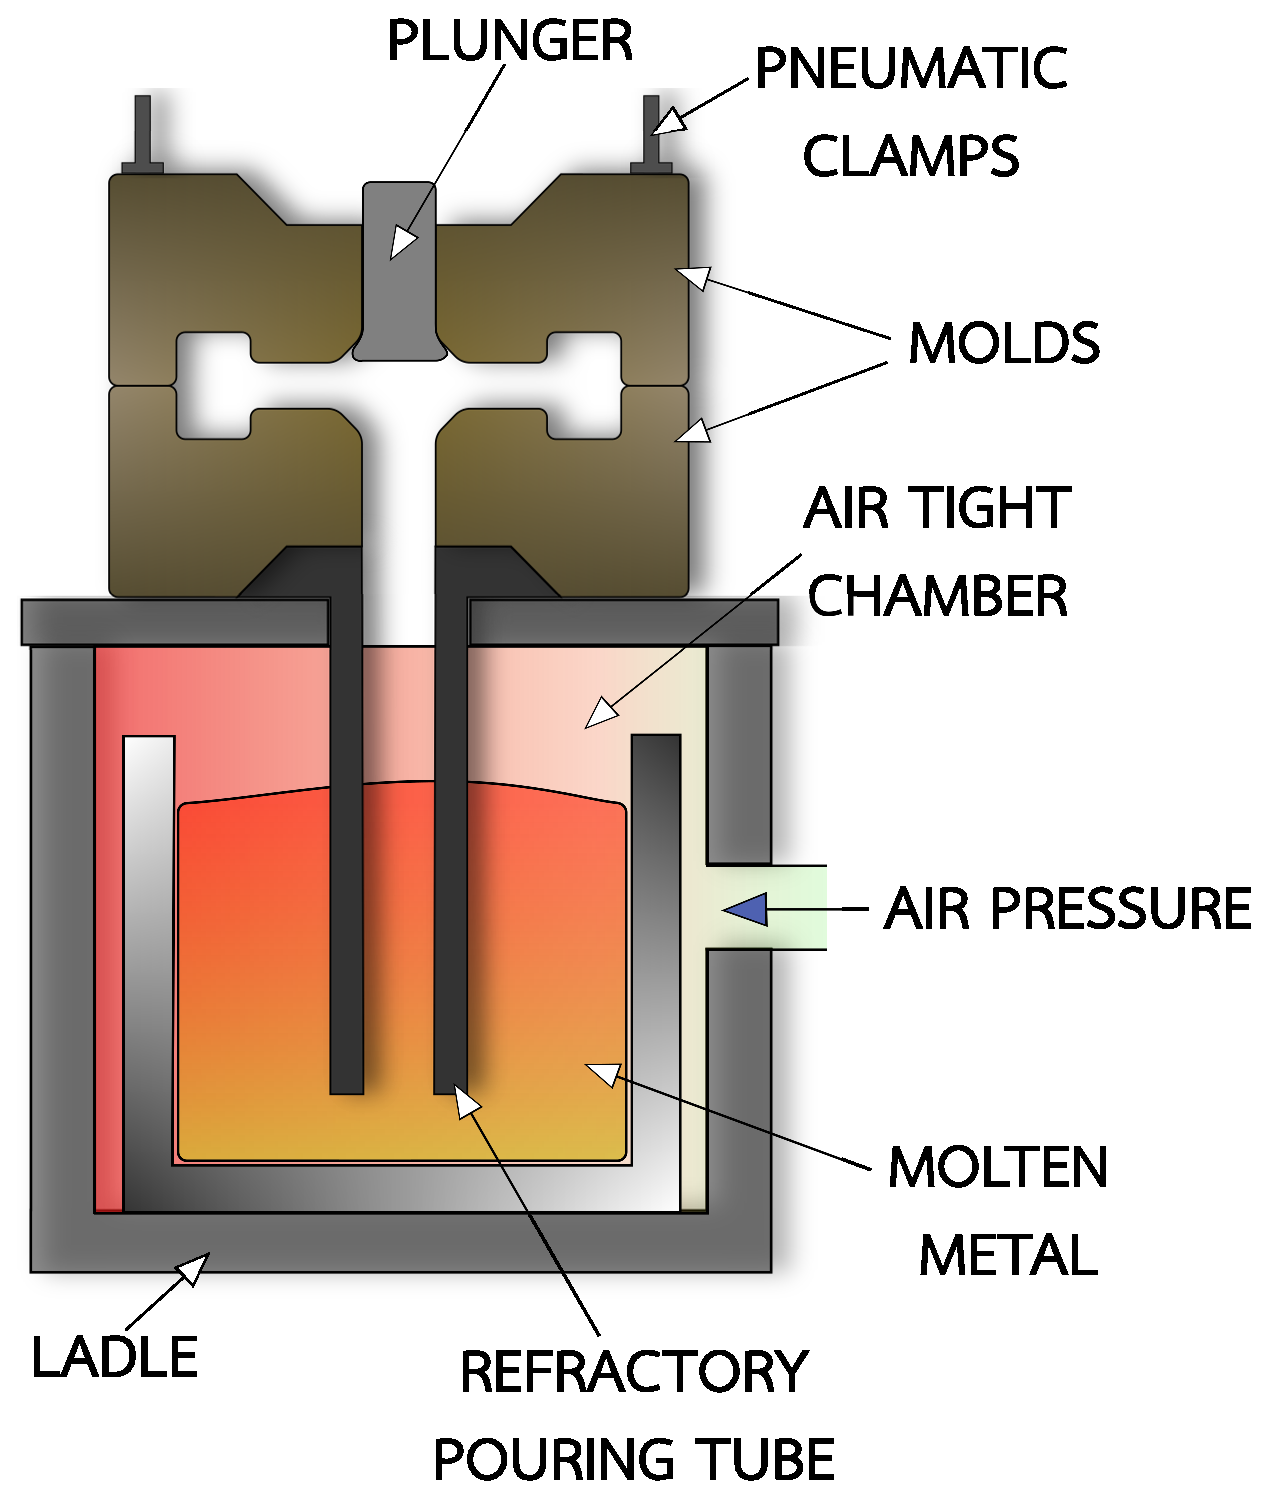
\includegraphics[width=0.45\textwidth]{Sources/pressurized_mold.eps}
        \caption{Schema di un casting in low-pressure permanent mold \autocite{Inkscape}}
    \end{figure}


    Tra i metodi tradizionali, questa tecnica produttiva, che consiste nella solidificazione di metallo fuso
    in uno stampo dalla geometria prossima a quella desiderata, si é negli ultimi anni notevolmente evoluta
    al punto da essere il gold standard nella
    produzione di parti in superleghe di Nickel ad alte prestazioni, con tecniche avanzate come il casting con
    gas a bassa pressione o l' \textit{investment casting}, scelta definitiva per la manufattura del componente. 

    Altri processi quali ad esempio il casting in lingotti, con successiva forgiatura o estrusione, se applicati a queste superleghe,
    portano troppo spesso a cricche e danni irreversibili durante la lavorazione \autocite{Mouritz}.

    Inoltre, seppur non sempre al livello della manufattura additiva, l'\textit{investment casting} consente comunque un minor spreco 
    di materiale, dato che le operazioni di natura strettamente sottrattiva sono limitate ad un'inevitabile
    rifinitura del componente estratto dallo stampo. 

    

    \clearpage

        \subsection{Solidificazione\label{Casting_solid}}

        


        \clearpage
        \subsection{Struttura\label{Casting_strutt}}

            \subsubsection{Zone fredde, colonnari e centrali\label{Casting_strutt_zone}}

            \begin{figure}[h!]
                \centering
                \phantomsection \label{grain_casting}
                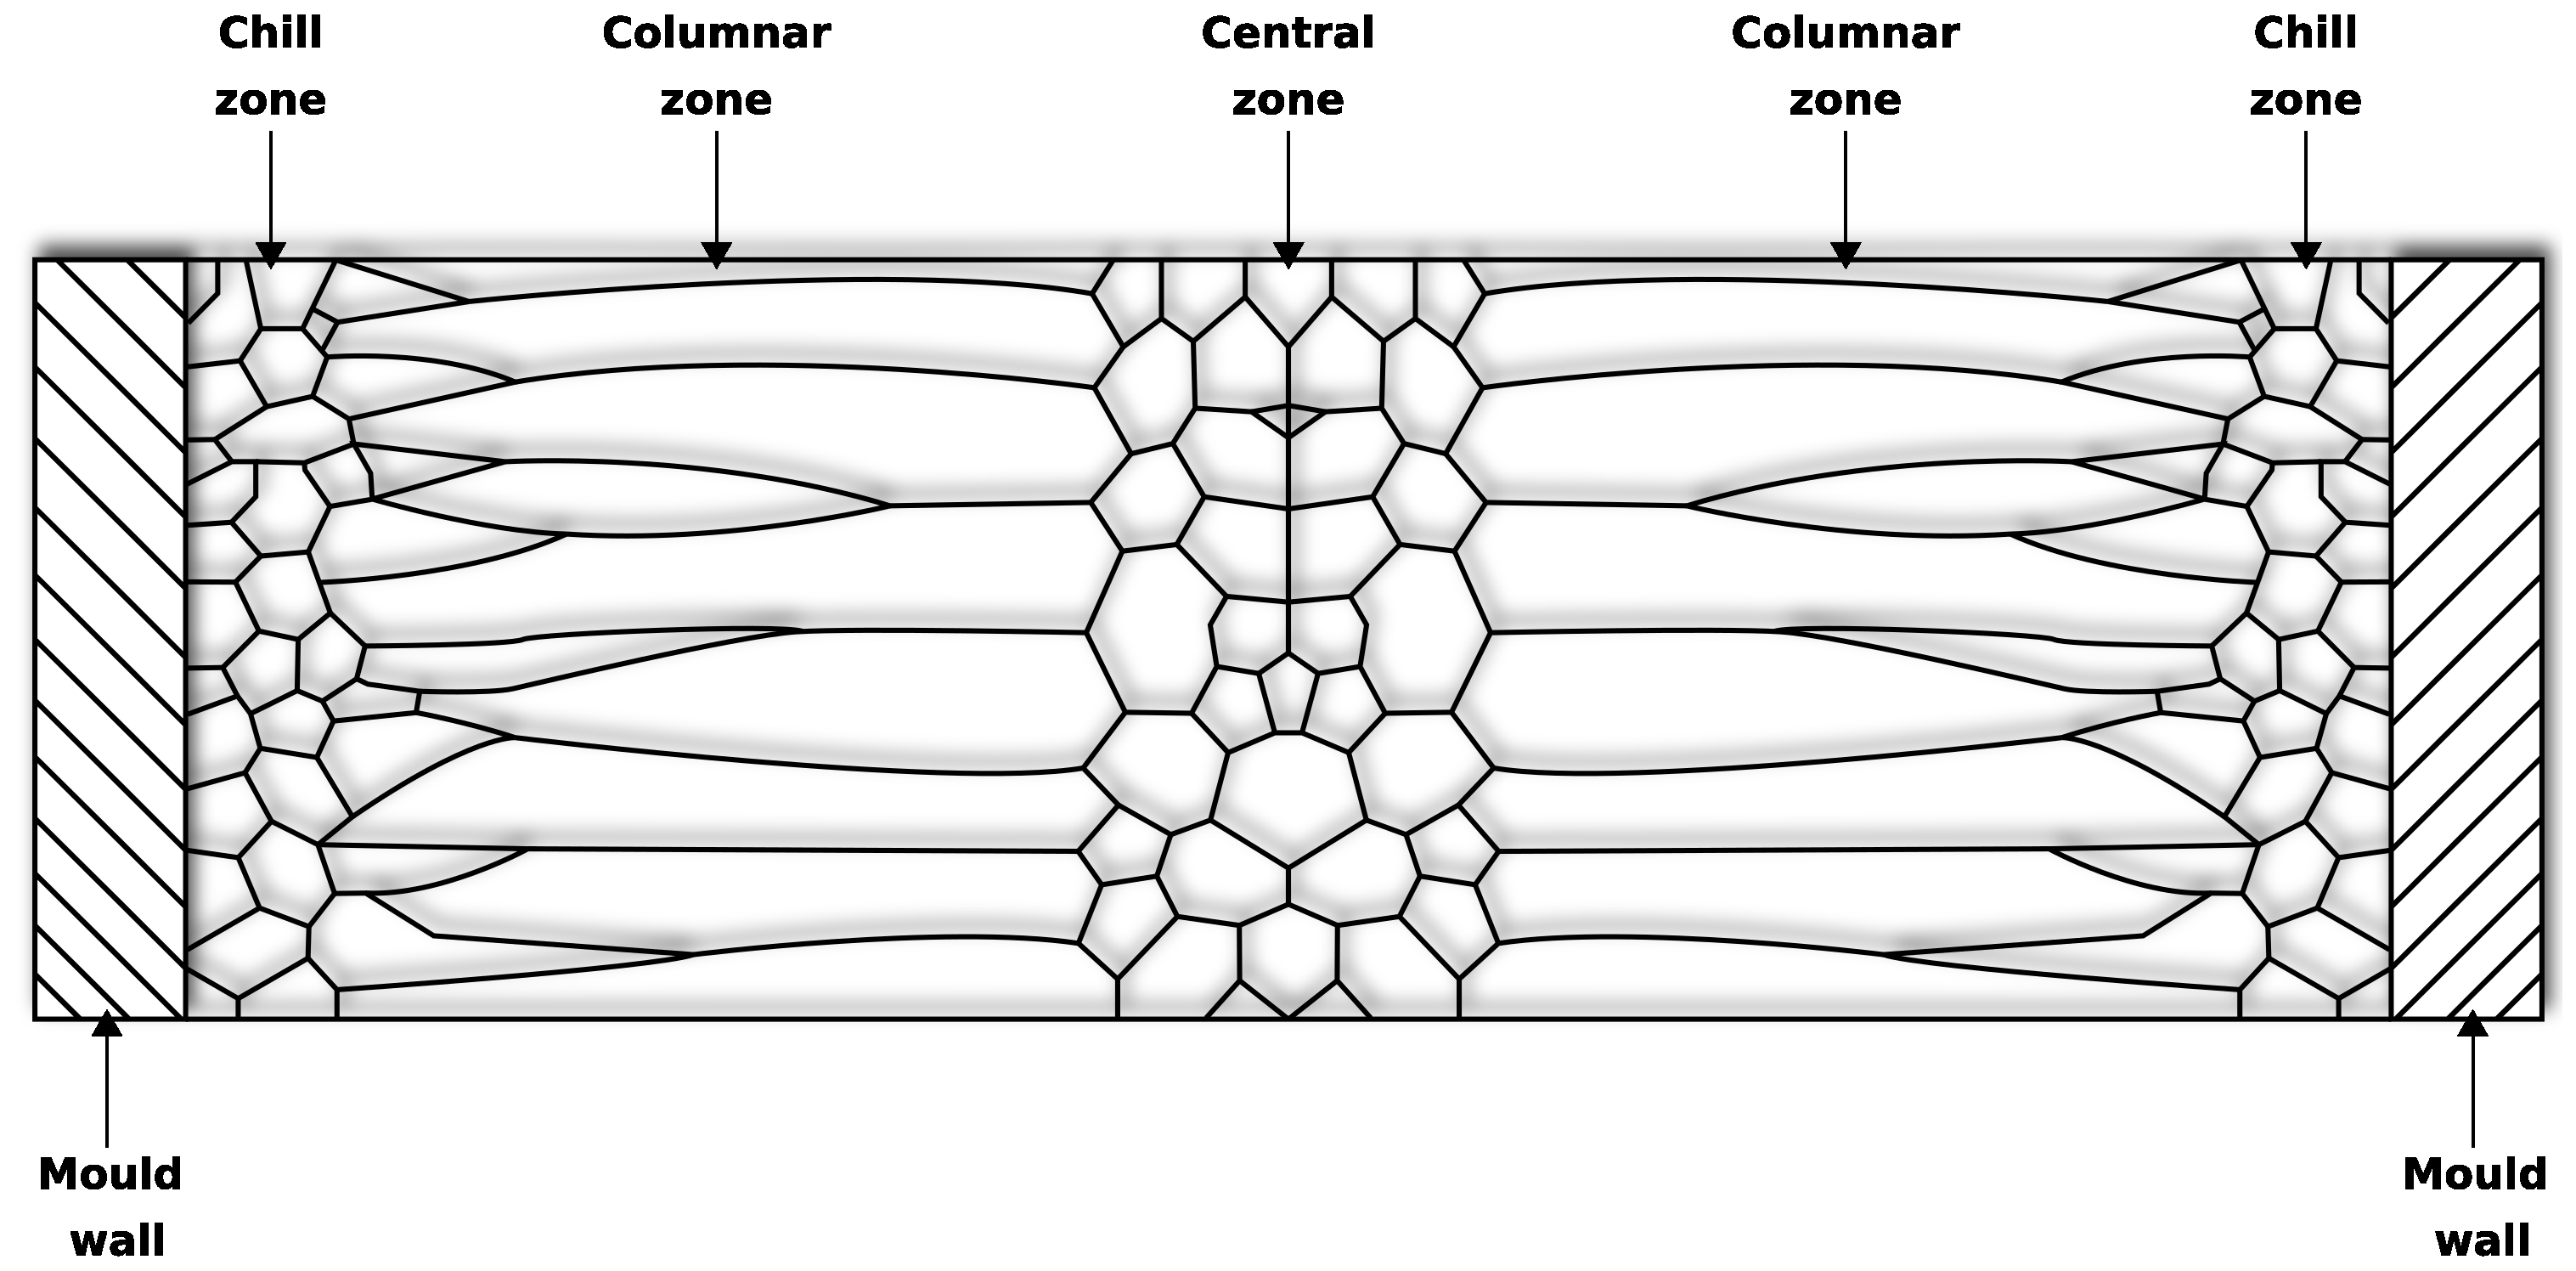
\includegraphics[width=\textwidth]{Sources/grain.eps}
                \caption{Grani di un lingotto raffreddato \autocite{Inkscape}}
            \end{figure}

            \clearpage 

            \subsubsection{Affinamento dei grani\label{Casting_strutt_affinamento}}


            \clearpage


        \subsection{Difetti\label{Casting_difetti}}


        \clearpage 

            \subsubsection{Porositá e ritiro\label{Casting_difetti_porosita}}

            \clearpage 

            \subsubsection{Inclusioni\label{Casting_difetti_inclusioni}}

            \clearpage 

            \subsubsection{Segregazione degli elementi di lega\label{Casting_difetti_segregazione}}
    
            \clearpage

        \subsection{Microfusione\label{Casting_microfusione}}



        \clearpage

    \section{Funzioni, obiettivi, vincoli\label{Funzioni_ob_vinc}}


    \clearpage 


    \section{Indici di merito\label{material_index}}

        Una buona strategia di analisi qualitativa per la selezione di materiali é rappresentata dalla valutazione di alcuni parametri frazionari, riferiti a una moltitudine di proprietá fisiche, chimiche, termiche, meccaniche, ecc, noti come indici di merito.
        
        Tali indici, definiti ad hoc in base alle necessitá del progettista, consentono di effettuare rapidamente un’indagine comparativa tra una lista di potenziali candidati che hanno superato una fase di preselezione, nel caso in cui la scelta del materiale non sia particolarmente ovvia o scontata. 
        \\ \\
        Nel caso specifico della paletta di uno stadio di turbina ad alta pressione, come giá visto in precedenza, sorgono diverse sfide con requisiti estremi da soddisfare simultaneamente.

        Possono quindi tornare molto utili alcuni indici di merito, dato che devono essere garantiti una elevata temperatura di esercizio, un basso coefficiente di espansione termica, un’alta fracture toughness, un’alta resistenza a fatica, un elevato modulo elastico, un’alta frequenza naturale di risonanza, oltre che un’ottima resistenza all’aggressivitá chimica dell’ambiente operativo. 
        
        Tutti i possibili indici di merito di un materiale sono spesso definiti in funzione della densitá, specialmente in campo aerospaziale, in cui l’ottimizzazione del peso di ogni componente risulta fondamentale, tra le svariate motivazioni, per massimizzare l’efficienza propulsiva, riducendo quindi la spesa sul carburante, che ha un impatto sostanziale sui costi complessivi di un velivolo.
        \\ \\ 
        In seguito alla promettente fase di preselezione sul database,
        superata da cinque materiali candidati, si é deciso di concentrarsi sugli indici relativi alla \textit{fracture toughness} e alla \textit{resist fatigue},
        per le quali i materiali preselezionati non mostrano evidenti compromessi ottimali.

        \begin{figure}[h!]
            \centering
            \phantomsection \label{blade_load}
            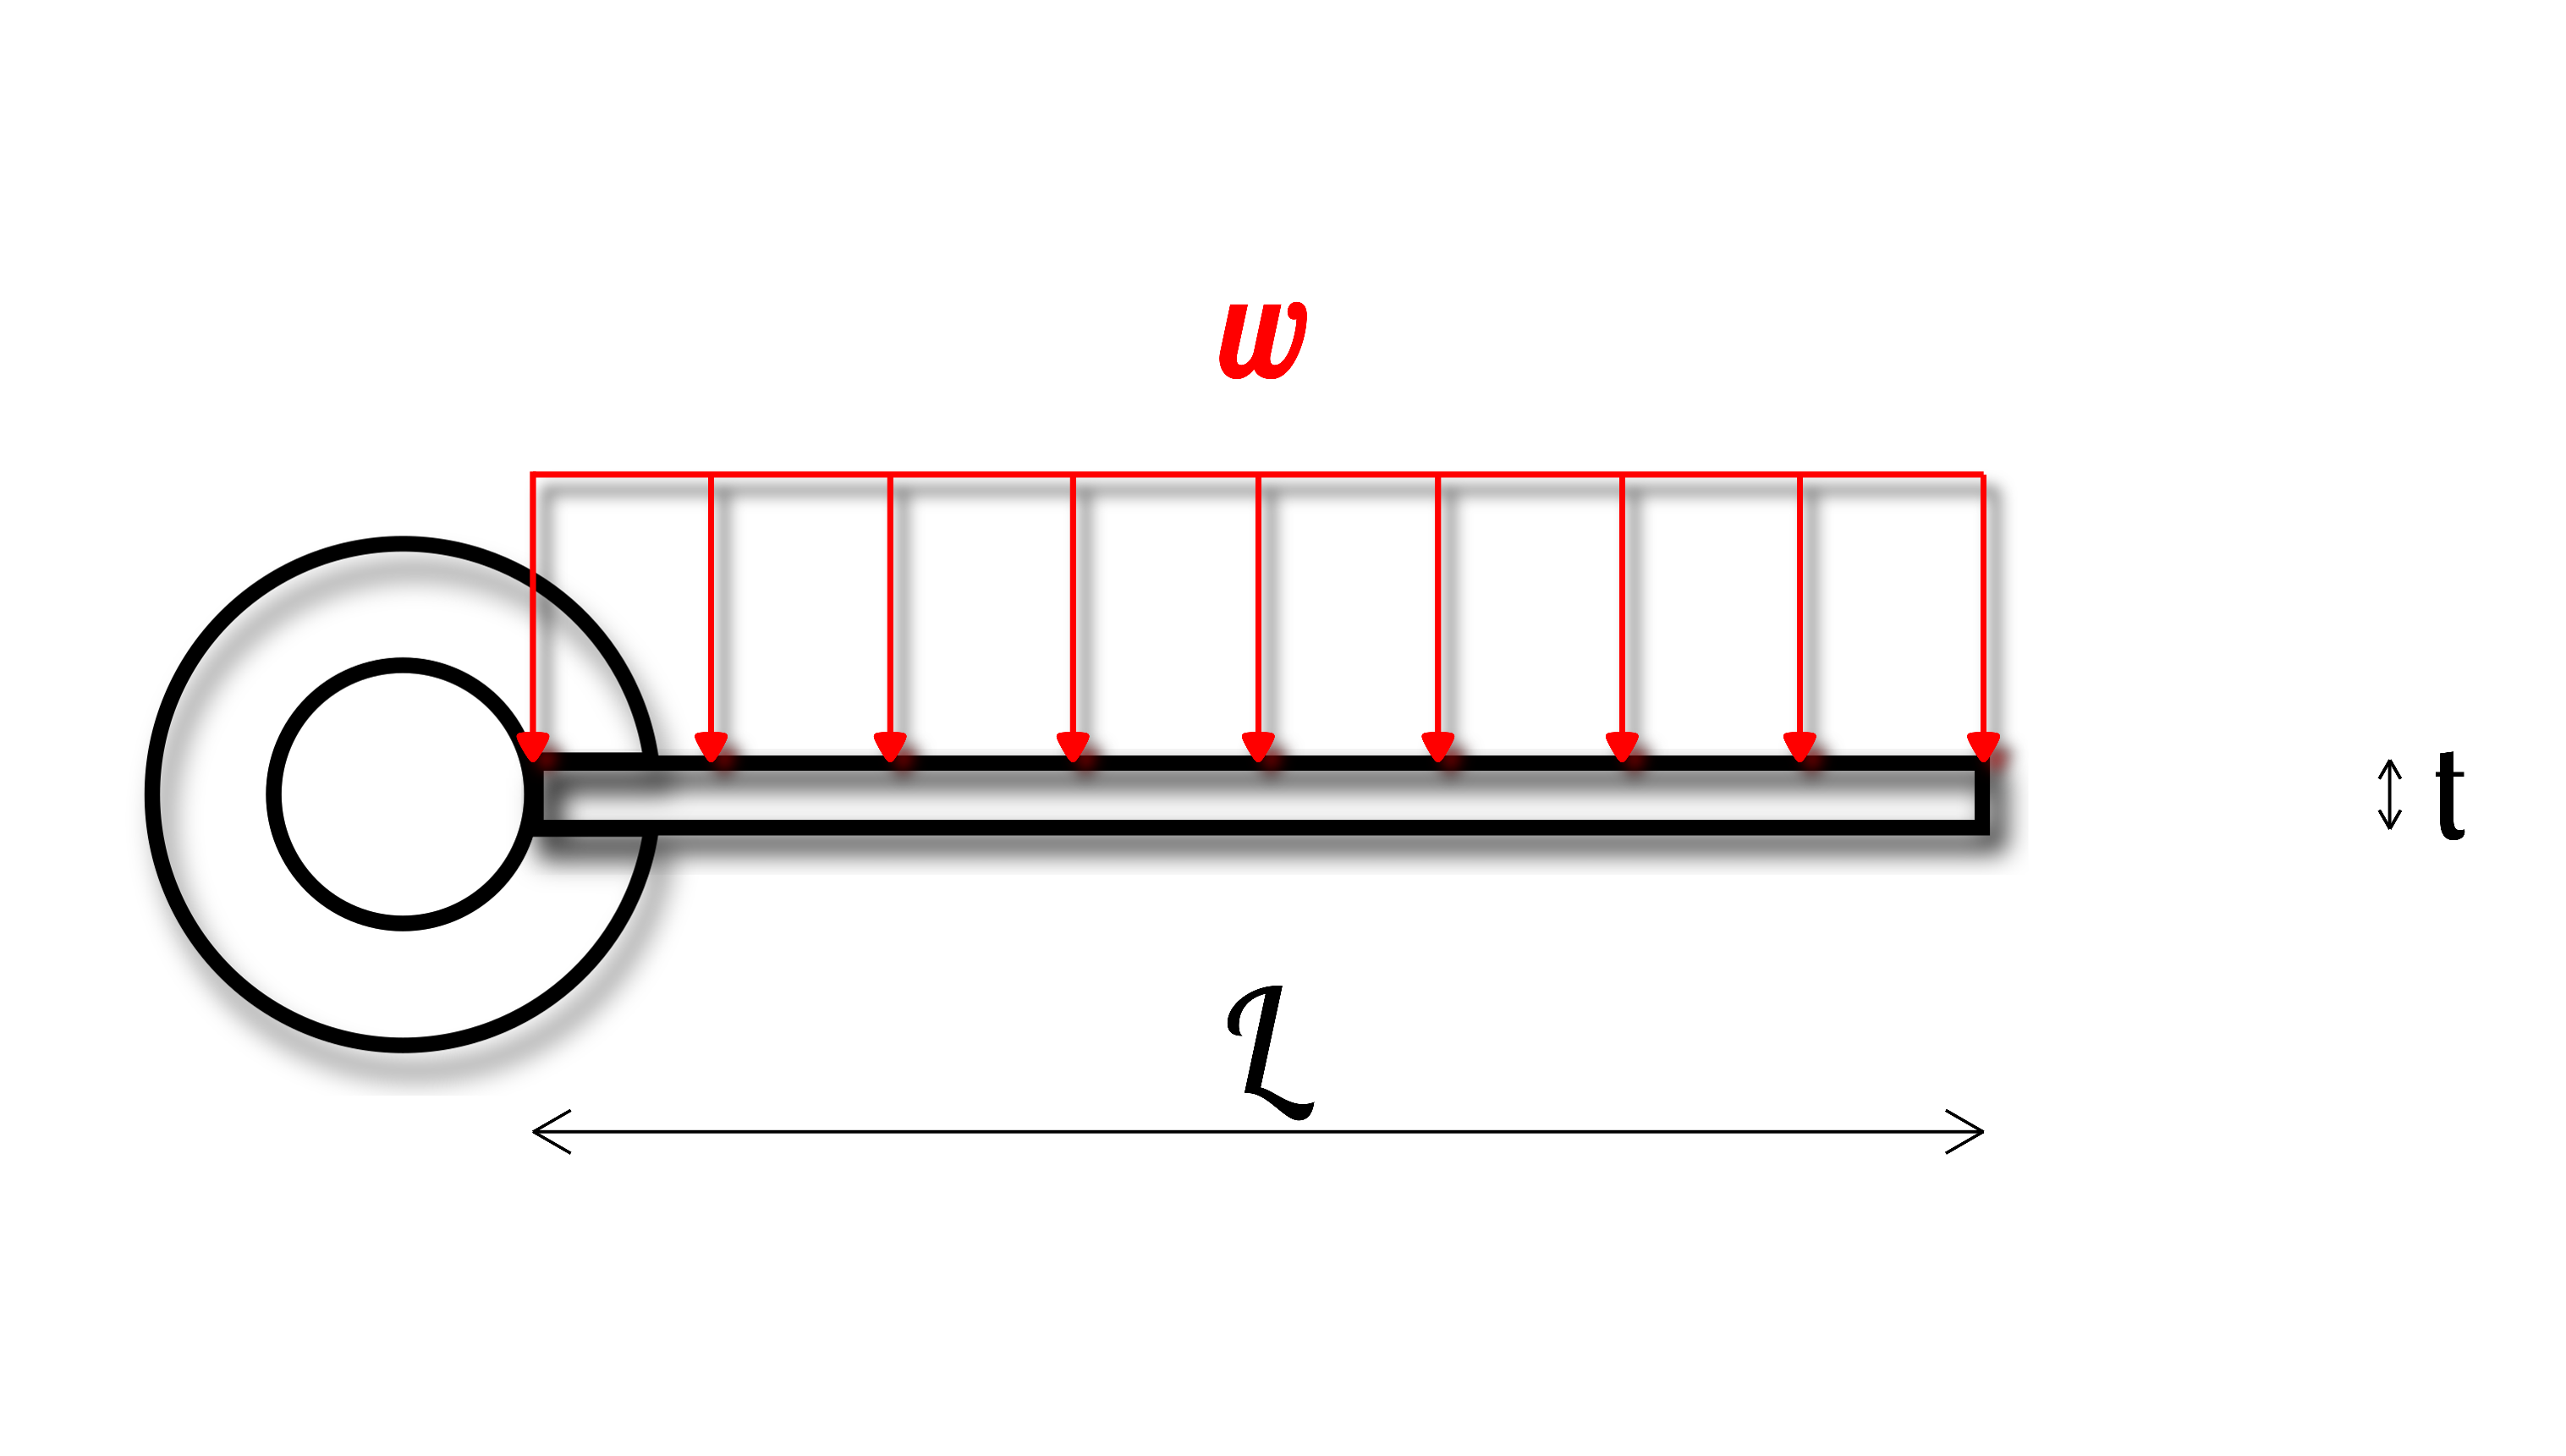
\includegraphics[width=0.8\textwidth]{Sources/blade_load.eps}
            \caption{Schematizzazione semplificata di una paletta \autocite{Inkscape}}
        \end{figure}
        \clearpage

        Per semplificare i calcoli, si assume una paletta rappresentata da una trave a base rettangolare
        estrusa, caratterizzata da:

        \begin{itemize}
            \item Lunghezza \textit{L} [m]
            \item Spessore \textit{t} [m]
            \item Larghezza $\lambda t \ [m]$ (con aspect ratio $\lambda$)
            \item Carico uniformemente distribuito $w = \frac{F}{L}$ [N/m]
            \item Stress applicato $\sigma(y) = \frac{M}{I} \cdot y \ \ \ [\frac{N}{m^2}]$ (dall'equazione di \textit{Navier})
                \begin{itemize}
                    \item $I = \frac{\alpha t^4}{12} \ \ [m^4]$ 
                    \item $M = \frac{wl^2}{2} \ \ [N \cdot m]$
                \end{itemize}
            \item Stress massimo per $\sigma_{max} = \sigma(y = \frac{t}{2})$
            \item Area della sezione $A = \lambda t^2 \ [m^2]$
            \item Densitá $\rho \ [\frac{kg}{m^3}]$
            \item Massa $m = \rho \cdot AL \ \ [kg]$
        \end{itemize}

        Attraverso una manipolazione delle giuste grandezze, gli indici di merito di interesse possono essere ricavati 
        in maniera del tutto indipendente dalla geometria della paletta, focalizzandosi quindi
        sulle proprietá intrinseche del materiale.
        \\ \\ 
        Ipotizzando che la paletta abbia una cricca centrale di dimensioni trascurabili
        rispetto alla sua larghezza, si definisce la \textit{fracture toughness}:

        \begin{equation}
            K_{1c} = \sigma\left(\pi c\right)^{0.5} 
            \phantomsection \label{equation:frac_tough}
        \end{equation}
        dove $\sigma$ é lo sforzo applicato, c é la dimensione della cricca. \\ \\ 

        Manipolando l'equazione con le caratteristiche della paletta precedentemente
        elencate, si ottiene una massa $m \propto \left(\frac{\rho}{K_{1c}}\right) $.

        Alla luce di quanto detto, si definisce il relativo indice di merito, da massimizzare \autocite{SciencePubGroup}:

        \begin{equation}
            i_{K} = \left (\frac{K_{1c}}{\rho}\right)
            \phantomsection \label{equation:index_frac_tough}
        \end{equation}
        \clearpage 

        Si procede in maniera del tutto analoga per definire un indice di merito relativo alla 
        \textit{resist fatigue}.

        Si definisce una \textit{resist fatigue} (che deve essere il piú alta possibile,
        visto l'onere delle sollecitazioni cicliche a cui é tipicamente sottoposta una paletta di turbina), 
        attraverso la disuguaglianza:

        \begin{equation}
            \sigma_e \geq \frac{wL}{A}
            \phantomsection \label{equation:resist_fatigue}
        \end{equation}

        Dopo varie sostituzioni algebriche, si ottiene una massa $m \propto \frac{\rho}{\sigma_e}$.

        Per cui in definitiva, si definisce il relativo indice di merito, da massimizzare \autocite{SciencePubGroup}:

        \begin{equation}
            \phantomsection \label{equation:resist_fatigue_index}
            i_{sigma} = \left (\frac{\sigma_e}{\rho}\right)
        \end{equation}

        Sfruttando queste definizioni ed i dati reperiti su \textit{Granta}, 
        sono stati calcolati i due indici di merito per ogni materiale, tramite un breve script in 
        \textit{Octave} \autocite{Octave}, disponibile nel repository di questo progetto \autocite{Relazione_materiali}. \\ 

        Considerando che, per come sono stati definiti, tali indici devono essere massimizzati al fine di ridurre il peso, 
        una possibile opzione é quella di comparare il valore massimo di ognuno dei due indici e trovare un compromesso
        a seconda delle prioritá di progetto.

        \begin{equation}
            Materials = [MARM432, \ IN162, \ IN738C, \ IN738LC, \ MARM421] 
            \phantomsection \label{vector:material_list}
        \end{equation}

        \begin{equation}
            \vec{i}_{sigma} = [\textbf{0.0069325}, \ 0.0053870, \  0.0061420,
             \ 0.0039815, \  0.0060681
            ]
            \phantomsection \label{vector:index_fatigue}
        \end{equation}

        \begin{equation}
            \vec{i}_{K} = [0.00046442,\   0.00055294,\   0.00047407,\
            \textbf{0.00057901},\   0.00039814]
            \phantomsection \label{vector:index_frac_tough}
        \end{equation}

        Da (\ref{vector:material_list}), (\ref{vector:index_fatigue}) e (\ref{vector:index_frac_tough}) si evince come 
        la lega \textit{MARM432} presenti la migliore resistenza a fatica per peso, permettendo, potenzialmente, 
        una maggiore durata dell'operativitá del componente.

        D'altro canto, si evince anche che la lega \textit{IN738LC}

        
        \clearpage


    \section{Conclusioni\label{conclusioni}}

    \clearpage

    \printbibliography
    
\end{document}
